\documentclass[
  captions=tableheading,
  bibliography=totoc, 
  titepage=firstiscover,
]{scrartcl}

\usepackage{blindtext} %neuer input

\usepackage{longtable} % Tabellen über mehrere Seiten

\usepackage[utf8]{inputenc} %neuer input

\usepackage{scrhack}

\usepackage[aux]{rerunfilecheck} %Warnung falls nochmal kompiliert werden muss

\usepackage{fontspec} %Fonteinstellungen

\recalctypearea{}

\usepackage[main=ngerman]{babel} %deutsche Spracheinstellung

\usepackage{ragged2e} %neuer input

\usepackage{amsmath, nccmath}

\usepackage{amssymb} %viele mathe Symbole

\usepackage{mathtools} %Erweiterungen für amsmath


\DeclarePairedDelimiter{\abs}{\lvert}{\rvert}
\DeclarePairedDelimiter{\norm}{\lVert}{\rVert}

\DeclarePairedDelimiter{\bra}{\langle}{\rvert}
\DeclarePairedDelimiter{\ket}{\lvert}{\rangle}

\DeclarePairedDelimiterX{\braket}[2]{\langle}{\rangle}{
#1 \delimsize| #2
}

\NewDocumentCommand \dif {m}
{
\mathinner{\symup{d} #1}
}


\usepackage[
  math-style=ISO,
  bold-style=ISO,
  sans-style=italic,
  nabla=upright,
  partial=upright,
  warnings-off={
    mathtools-colon,
    mathtools-overbracket,
  },
]{unicode-math}

\setmathfont{Latin Modern Math}
\setmathfont{XITS Math}[range={scr, bfscr}]
\setmathfont{XITS Math}[range={cal, bfcal}, StylisticSet=1]


\usepackage[
  locale=DE,
  separate-uncertainty=true,
  per-mode=reciprocal,
  output-decimal-marker={,},
]{siunitx}

\usepackage[autostyle]{csquotes} %richtige Anführungszeichen

\usepackage{xfrac}

\usepackage{float}

\floatplacement{figure}{htbp}

\floatplacement{table}{htbp}

\usepackage[ %floats innerhalb einer section halten
  section,   %floats innerhalb er section halten
  below,     %unterhalb der Section aber auf der selben Seite ist ok
]{placeins}

\usepackage[
  labelfont=bf,
  font=small,
  width=0.9\textwidth,
]{caption}

\usepackage{subcaption} %subfigure, subtable, subref

\usepackage{graphicx}

\usepackage{grffile}

\usepackage{booktabs}

\usepackage{microtype} %Verbesserungen am Schriftbild

\usepackage[
backend=biber,
]{biblatex}

\addbibresource{../lit.bib}

\usepackage[ %Hyperlinks im Dokument
  german,
  unicode,
  pdfusetitle,
  pdfcreator={},
  pdfproducer={},
]{hyperref}

\usepackage{bookmark}

\usepackage[shortcuts]{extdash}

%\usepackage{warpcol}


\begin{document}
    \title{V354 Gedämpfte und erzwungene Schwingungen}
    \author{  
    Tobias Rücker\\
    \texorpdfstring{\href{mailto:tobias.ruecker@tu-dortmund.de}{tobias.ruecker@tu-dortmund.de}
    \and}{,} 
    Paul Störbrock\\
    \texorpdfstring{\href{mailto:paul.stoerbrock@tu-dortmund.de}{paul.stoerbrock@tu-dortmund.de}}{}
    }
    \date{Durchführung: 26.11.2019, Abgabe: 03.12.2019\vspace{-4ex}}
\maketitle
\center{\Large Versuchsgruppe: \textbf{42}}
    
    \begin{abstract}
    \centering
        \textbf{Ziel:} Bestimmung des Dämpfungswiderstandes eines LRC-Kreises. 
    \end{abstract}

\newpage
\tableofcontents
\newpage

% Theorie %%%%%%%%%%%%%%%%%%%%%%%%%%%%%%%%%%%%%%%%%%%%%%%%%%%%%%%%%%%%%%%%%%%%%%%%%%%%%%%%%%%%%%%%%%%%%%%%%%%%%%%%%%%%%%%%%%%%%%%%%%%%%%%%%%%%%%%%%%%

\section{Theorie}\justifying
\begin{align}
\intertext{Ein Schwingkreis beschreibt einen Schaltkreis bestehend aus einem
Kondensator und einer Spule. Die Spule besitzt dabei die Induktivität $L$ und der
Kondensator die Kapazität $C$. Wird auf diese Schaltung nun eine Spannung $U_0$ 
gegeben, so oszilliert die Spannung beim Schwingkreis ungedämpft. 
Wird nun ein Widerstand in die Schaltung eingebaut, so verliert das System mit der
Zeit Energie, die in Form von joulscher Wärme an den Widerstand irreversibel
übertragen wird. Dadurch verläuft die Amplitude der Spannung mit der Zeit gegen 0.
Die zeitliche Veränderung der Stromstärke kann dabei durch folgende Formel
beschrieben werden \cite{V354}:}
\symbffrak{I}(t) &= \symbffrak{U}_1e^ {i\tilde{\omega}_1 t}+\symbffrak{U}_2 e^{i \tilde{\omega}_2 t} \text{, wobei}\\
\tilde{\omega} _{1,2} &= i\frac{R}{2L} \pm \sqrt{\frac{1}{LC}-\frac{R^2}{4L^2}} \text{ist.} \label{eq:omega}\\
\intertext{Aus diesem Zusammenhang ergeben sich drei verschiedene Fälle.
Der erste Fall beschreibt, dass \cite{V354}}
\frac{1}{LC} & < \frac{R^2}{4L^2} \label{eq:Fall1}
\intertext{ist und damit der Wurzelterm von $\tilde{\omega}$ \eqref{eq:omega} komplex wird.
Die zugehörige Schwingungsgleichung entspricht damit \cite{V354}}
    I(t)&=A_0 e^{-2 \pi \mu t} \cos (2 \pi \nu t + \eta) \label{eq:I}.
\end{align}
\justifying
Dabei beschreiben die Terme $2 \pi \nu$ und $2 \pi \mu$ jeweils
\begin{align}
  2 \pi \nu &= \sqrt{\frac{1}{LC}-\frac{R^2}{4L^2}} \; \text{und}\\
  2 \pi \mu &= \frac{R}{2L},
\end{align}
wobei $\nu$ die Frequenz ist.
Diese Gleichung beschreibt eine gedämpfte Schwingung. Die Amplitude $A_0$ läuft dabei
exponentiell gegen null.
Die Schwingungsdauer lässt sich dabei für diesen Fall schreiben als \cite{V354}:
\begin{align}
    T_0 &\phantom{:}=\frac{2 \pi}{\omega _0}=2 \pi \sqrt{LC} \text{, wobei sich nach einer Zeit $T_{ex}$ mit}\\
    T_{ex}&:= \frac{1}{2 \pi \mu}=\frac{2L}{R} \label{eq:Abkling}
\end{align}
\justify
die Spannungsamplitude um den Faktor $\sfrac{1}{e}$ verringert hat.
$T_{ex}$ wird daher auch Ablinkdauer genannt.
\justify
Der zweite Fall \cite{V354}
\begin{align}
    \frac{1}{LC} >\frac{R^2}{4L^2} \label{eq:Fall2}
\end{align}
stellt den Kriechfall dar. Bei diesem verschwindet der oszillatorische Teil und
die Wurzel aus Gleichung \eqref{eq:omega} wird positiv.
Die Funktion geht mit maximal einem Nulldurchgang nicht-oszillatorisch gegen null.
Ob ein Nulldurchgang sattfindet hängt dabei von den Anfangsbedingungen ab.
\newpage
\justify
Der dritte Fall stellt einen Spezialfall des zweiten dar.
Bei diesem lautet die Bedingung \cite{V354} wie folgt:
\begin{align}
    \frac{1}{LC} = \frac{R^2}{4L^2} \label{eq:Fall3}
\end{align}
Dieser wird der aperiodische Grenzfall genannt. Bei diesem kehrt die Kurve
am schnellsten zur Null zurück.\\
Neben gedämpften Schwingungen treten auch häufig erzwungene Schwingungen auf,
die hier durch eine sinusförmige Wechselpannung realisiert wird. 
Die Frequenzabhängigkeit des Kondensators wird dabei durch 
\begin{align}
    U_C (\omega)=\frac{U_0}{\sqrt{(1-LC\omega ^2)^2+\omega ^2 R^2 C^2}} \label{eq:9}
\end{align}
beschrieben.
Dabei ist zu bemerken, dass diese Funktion ein Maximum besitzt, welches die
angelegte Spannungsamplitude $U_0$ übersteigen kann.\\
Diese Frequenz wird im Allgemeinen als Resonanzfrequenz $\omega_{res}$ \cite{V354} 
\begin{align}
    \omega_{res} = \sqrt{\frac{1}{LC}-\frac{R^2}{2L^2}} \label{eq:omegares}
\end{align}
bezeichnet.\\
Aus dieser Formel können zwei Spezialfälle betrachtet werden.
Für den ersten Fall wird die schwache Dämpfung betrachtet \cite{V354}:
\begin{align}
    \frac{1}{LC} \gg \frac{R^2}{4L^2} \label{eq:Fall1b}
\end{align}
Der Faktor $\sfrac{1}{\omega _0 RC}$ beschreibt in diesem Fall, um welchen Faktor 
$U_{C,\text{max}}$ die Spannung $U_0$ übersteigt. Daher wird er auch als Güte 
oder Resonanzüberhöhung q bezeichnet.
Eine andere Beschreibung von q lässt sich mit der Breite der 
Resonanzkurve finden \cite{V354}:
\begin{align}
    q = \frac{\omega _0}{\omega _+ - \omega _-} \label{eq:guete}
\end{align}
Dabei beschreiben $\omega _+$ und $\omega _-$ die Breite der Resonanzkurve.
Sie beschreiben die Fequenzen, bei denen die Spannung auf die Größe 
$\sfrac{U_{C,\text{max}}}{\sqrt{2}}$ vom Maximum gesunken ist.
Die Breite der Resonanzkurve kann dabei durch
\begin{align}
    \omega _+ - \omega _- \approx \frac{R}{L} \label{eq:om+-}
\end{align}
approximiert werden.
\flushleft{Für }\justifying den Fall der starken Dämpfung \cite{V354}
\begin{align}
    \frac{1}{LC} \ll \frac{R^2}{4L^2} \label{eq:Fall2b}
\end{align}
existiert keine Resonanzüberhöhung mehr. 
Die frequenzabhängige Phasenverschiebung \cite{V353}
\begin{align}
    \varphi(\nu) &= \frac{\Delta T}{T} \cdot 2 \pi \quad &\text{mit} \; T &= \frac{1}{\nu} \label{eq:nu}\\
    \intertext{oder auch}
    \varphi(\nu)&=\arctan \left(-\frac{\omega R C}{1-LC \omega ^2}\right) \label{eq:phi}
\end{align}
zeigt, dass sich dabei der Wert $\sfrac{\pi}{2}$ bei \cite{V354}
\begin{align}
    \omega _0^2 &= \frac{1}{LC} \label{eq:omega0}
\intertext{ergibt. Wird $\omega _0 $ um $\pm\sfrac{\pi}{4}$ verschoben, so ergeben sich die Werte \cite{V354}}
    \omega_{1,2} &= \pm \frac{R}{2L} + \sqrt{\frac{R^2}{4L^2} + \frac{1}{LC} } \label{eq:om12}
\intertext{für $\omega _1$ und $\omega _2$. Daraus lässt sich die Beziehung \cite{V354}}
    \omega _1 - \omega _2 &= \frac{R}{L} \label{eq:omdiff}
\end{align}
herleiten.

% Fehlerrechnung %%%%%%%%%%%%%%%%%%%%%%%%%%%%%%%%%%%%%%%%%%%%%%%%%%%%%%%%%%%%%%%%%%%%%%%%%%%%%%%%%%%%%%%%%%%%%%%%%%%%%%%%%%%%%%%%%%%%%%%%%%%%%%%%%%%%%%%%%%%

\section{Fehlerrechnung}

Für die Auswertung werden die folgenden Formeln zur Bestimmung der eventuell anfallenden Fehler benötigt:
\begin{subequations}    
\begin{align}
    \intertext{Der Mittelwert wird berechnet mit folgender Formel:}
        \overline{x} &= \frac{1}{N}\sum_{i=1}^{N} x_i \label{eq:mittelw}
    \intertext{Um den Fehler des Mittelwerts zu bestimmen, wird}
        \Delta\overline{x} &= \frac{1}{\sqrt{N}} \sqrt{\frac{1}{1-N} \sum_{i=1}^{N} (x_i - \overline{x})^2} \label{eq:fmittelw}
    \intertext{verwendet. Für die gaußsche Fehlerfortpflanzung wird die folgende Gleichung benutzt:}
        \Delta f &= \sqrt{\sum_{i=1}^{N} \left( \frac{\delta f}{\delta x_i} \right)^2 \cdot (\Delta x_i)^2} \label{eq:ffort}
    \intertext{In der Auswertung selbst wird die Fehlerrechnung mithilfe von Pyhtonbefehlen \cite{uncertainties} durchgeführt.
    Für die lineare und nichtlineare Ausgleichsrechnung werden folgende Funktionen benötigt:}
        y &= m \cdot x + b\\
        m &= \frac{\overline{xy} - \overline{x} \cdot \overline{y}}{\overline{x^2} - {\overline{x}}^2}  \qquad \qquad
        b = \frac{\overline{y} \cdot \overline{x^2} - \overline{xy} \cdot \overline{x}}{\overline{x^2} - {\overline{x}}^2}
\end{align}
\end{subequations}

% Versuchsaufbau %%%%%%%%%%%%%%%%%%%%%%%%%%%%%%%%%%%%%%%%%%%%%%%%%%%%%%%%%%%%%%%%%%%%%%%%%%%%%%%%%%%%%%%%%%%%%%%%%%%%%%%%%%%%%%%%%%%%%%%%%%%%%%%%%%%%%%%%%%%

\section{Versuchsaufbau}\justifying
Benötigt werden: \textit{Ein Generator mit einem Innenwiderstand von $\SI{2.5}{\ohm}$, 
ein analoges Zweikanal-Oszilloskop, ein LRC-Glied mit drei ohmschen Widerständen 
($R_1 < R_2$), wovon einer der Widerstände ($R_3$) variabel sein soll, 
zwei BNC-Kabel, eine BNC-Steckverbindung und einen Tastkopf}.\\
Zuerst wird die BNC-Steckverbindung an dem Generator angebracht. 
Dann wird die Steckverbindung mit einem der Widerstände des LRC-Glieds und mit dem zweiten 
Eingang des Oszilloskops verbunden.
Zuletzt wird das LRC-Glied über einem BNC-Kabel mit Tastkopf 
mit dem ersten Eingang des Oszilloskops verbunden.

% Versuchsdurchführung %%%%%%%%%%%%%%%%%%%%%%%%%%%%%%%%%%%%%%%%%%%%%%%%%%%%%%%%%%%%%%%%%%%%%%%%%%%%%%%%%%%%%%%%%%%%%%%%%%%%%%%%%%%%%%%%%%%%%%%%%%%%%%%%%%%%%%%%%%%

\section{Versuchsdurchführung}\justifying

 \begin{enumerate}

    \item[a)] \justifying Zu Beginn wird am Generator eine Frequenz von 100Hz 
    eingestellt und eine Erregerspannung von 10V eingestellt. Danach wird der 
    Generator mit dem kleineren der festen Widerstände verbunden.
    Um die lineare Ausgleichsrechnung der Einhüllenden zu bestimmen, wird
    ein Bild vom Oszilloskop angefertigt aus dem dann Messwerte entnommen werden
    können.

    \item[b)] \justifying Um den Widerstand $R_{\text{ap}}$ zu bestimmen, wird der Generator 
    an den maximal eingestellten variablen Widerstand angeschlossen. Anschließend wird 
    der variable Widerstand reduziert, bis am Oszilloskop eine Überschwingung erkennbar 
    wird. Daraufhin wird der Widerstand stetig erhöht bis die Überschwingung verschwindet 
    und der Wert des Widerstandes notiert.
  
    \item[c)] \justifying Dann wird für die Messung der Frequenzabhängigkeit
                          der größere Widerstand von $\SI{271.6\pm 0.2}{\ohm}$ angeschlossen.
                          Daraufhin werden ungefähr 20 Werte für die Verschiebung der Nulldurchgänge 
                          und Frequenz in gleichmäßigem Abstand um die 
                          Resonanzfrequenz gemessen und datiert. Dafür wird das Oszilloskop so eingestellt, 
                          dass die Kurve für Generatorspannung und Spannung des Schwingkreises zu sehen sind.
 \end{enumerate}
 \newpage
% Auswertung %%%%%%%%%%%%%%%%%%%%%%%%%%%%%%%%%%%%%%%%%%%%%%%%%%%%%%%%%%%%%%%%%%%%%%%%%%%%%%%%%%%%%%%%%%%%%%%%%%%%%%%%%%%%%%%%%%%%%%%%%%%%%%%%%%%%%%%%%%%

\section{Auswertung}\justifying

%Auswertung 5a ----------------------------------------------------------------------------------------------------------------------------------------

  Die Kurven in den Bildern \ref{fig:R1} und \ref{fig:R2} spiegeln das Dämpfungsverhalten der einzelnen Widerstände wieder. 
  Es ist erkennbar, dass die Schwingung in Bild \ref{fig:R2} stärker gedämpft wird, was darauf schließen lässt, dass R2 der 
  größere der beiden Widerstände ist.

  \begin{figure}[H]
    \begin{subfigure}{0.495\linewidth}
     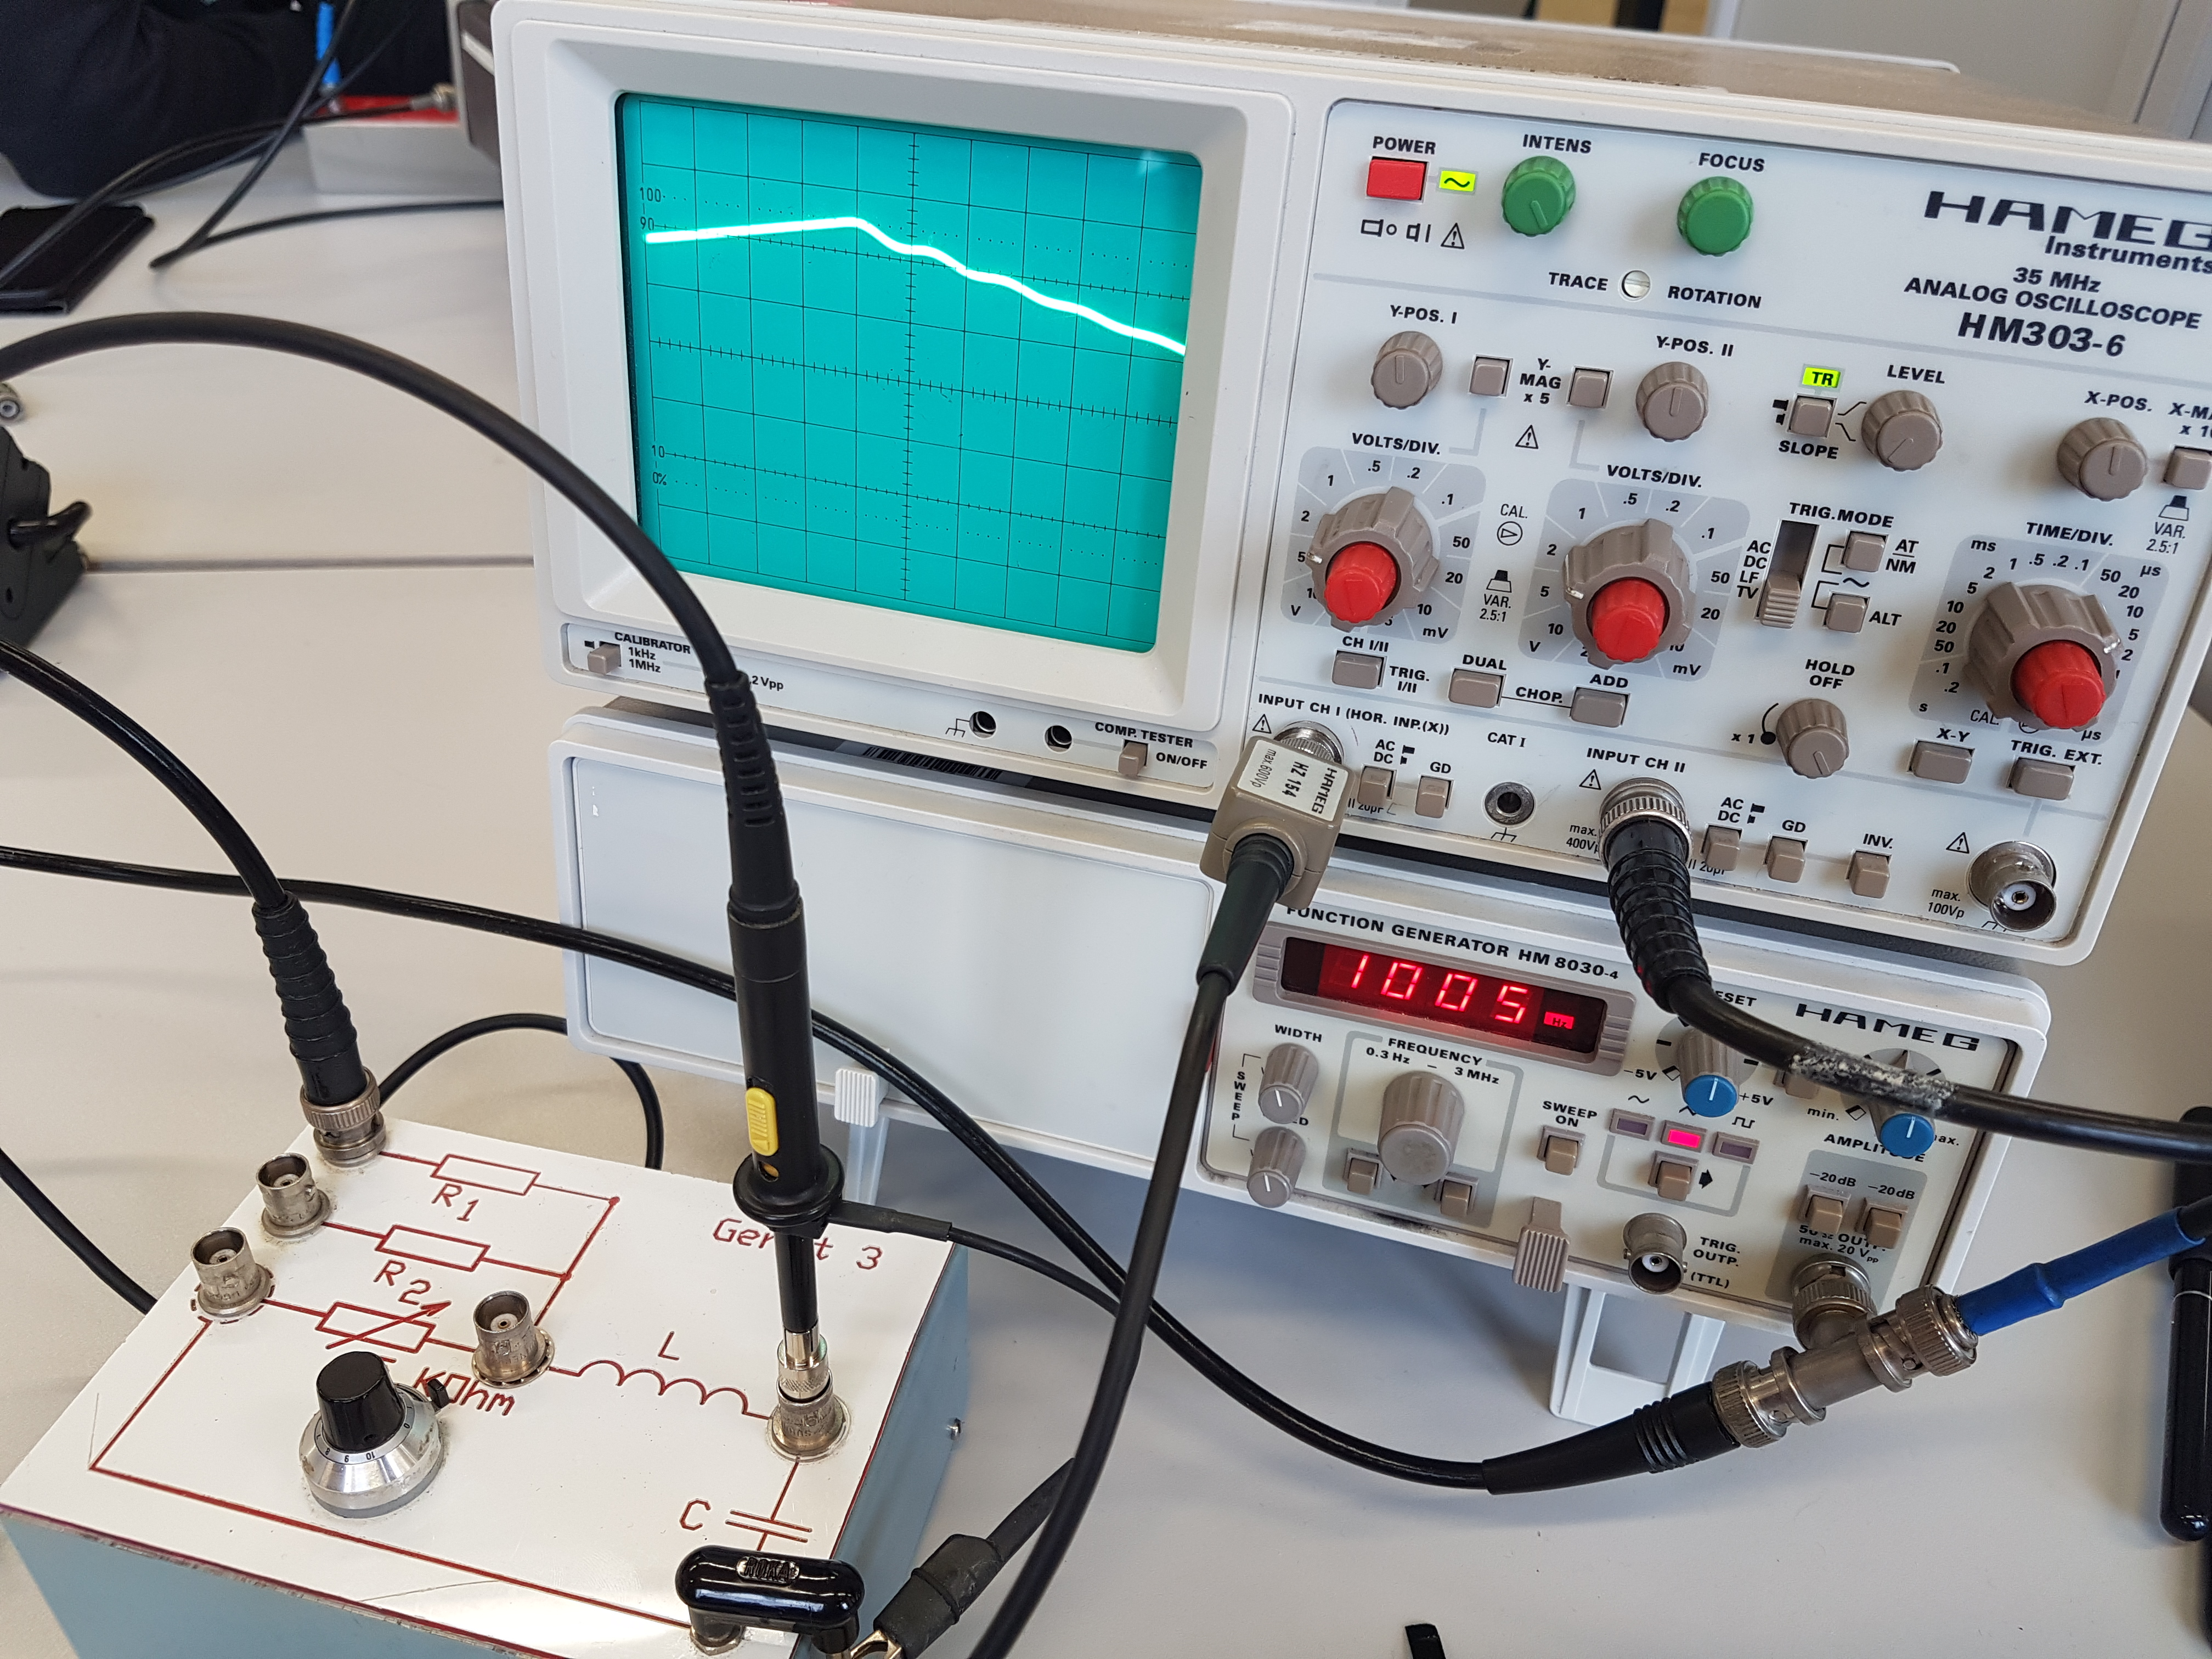
\includegraphics[width=\textwidth]{images/R1.jpg}
     \centering
     \caption{Widerstand R1}
     \label{fig:R1}
    \end{subfigure}
    \begin{subfigure}{0.495\linewidth}
     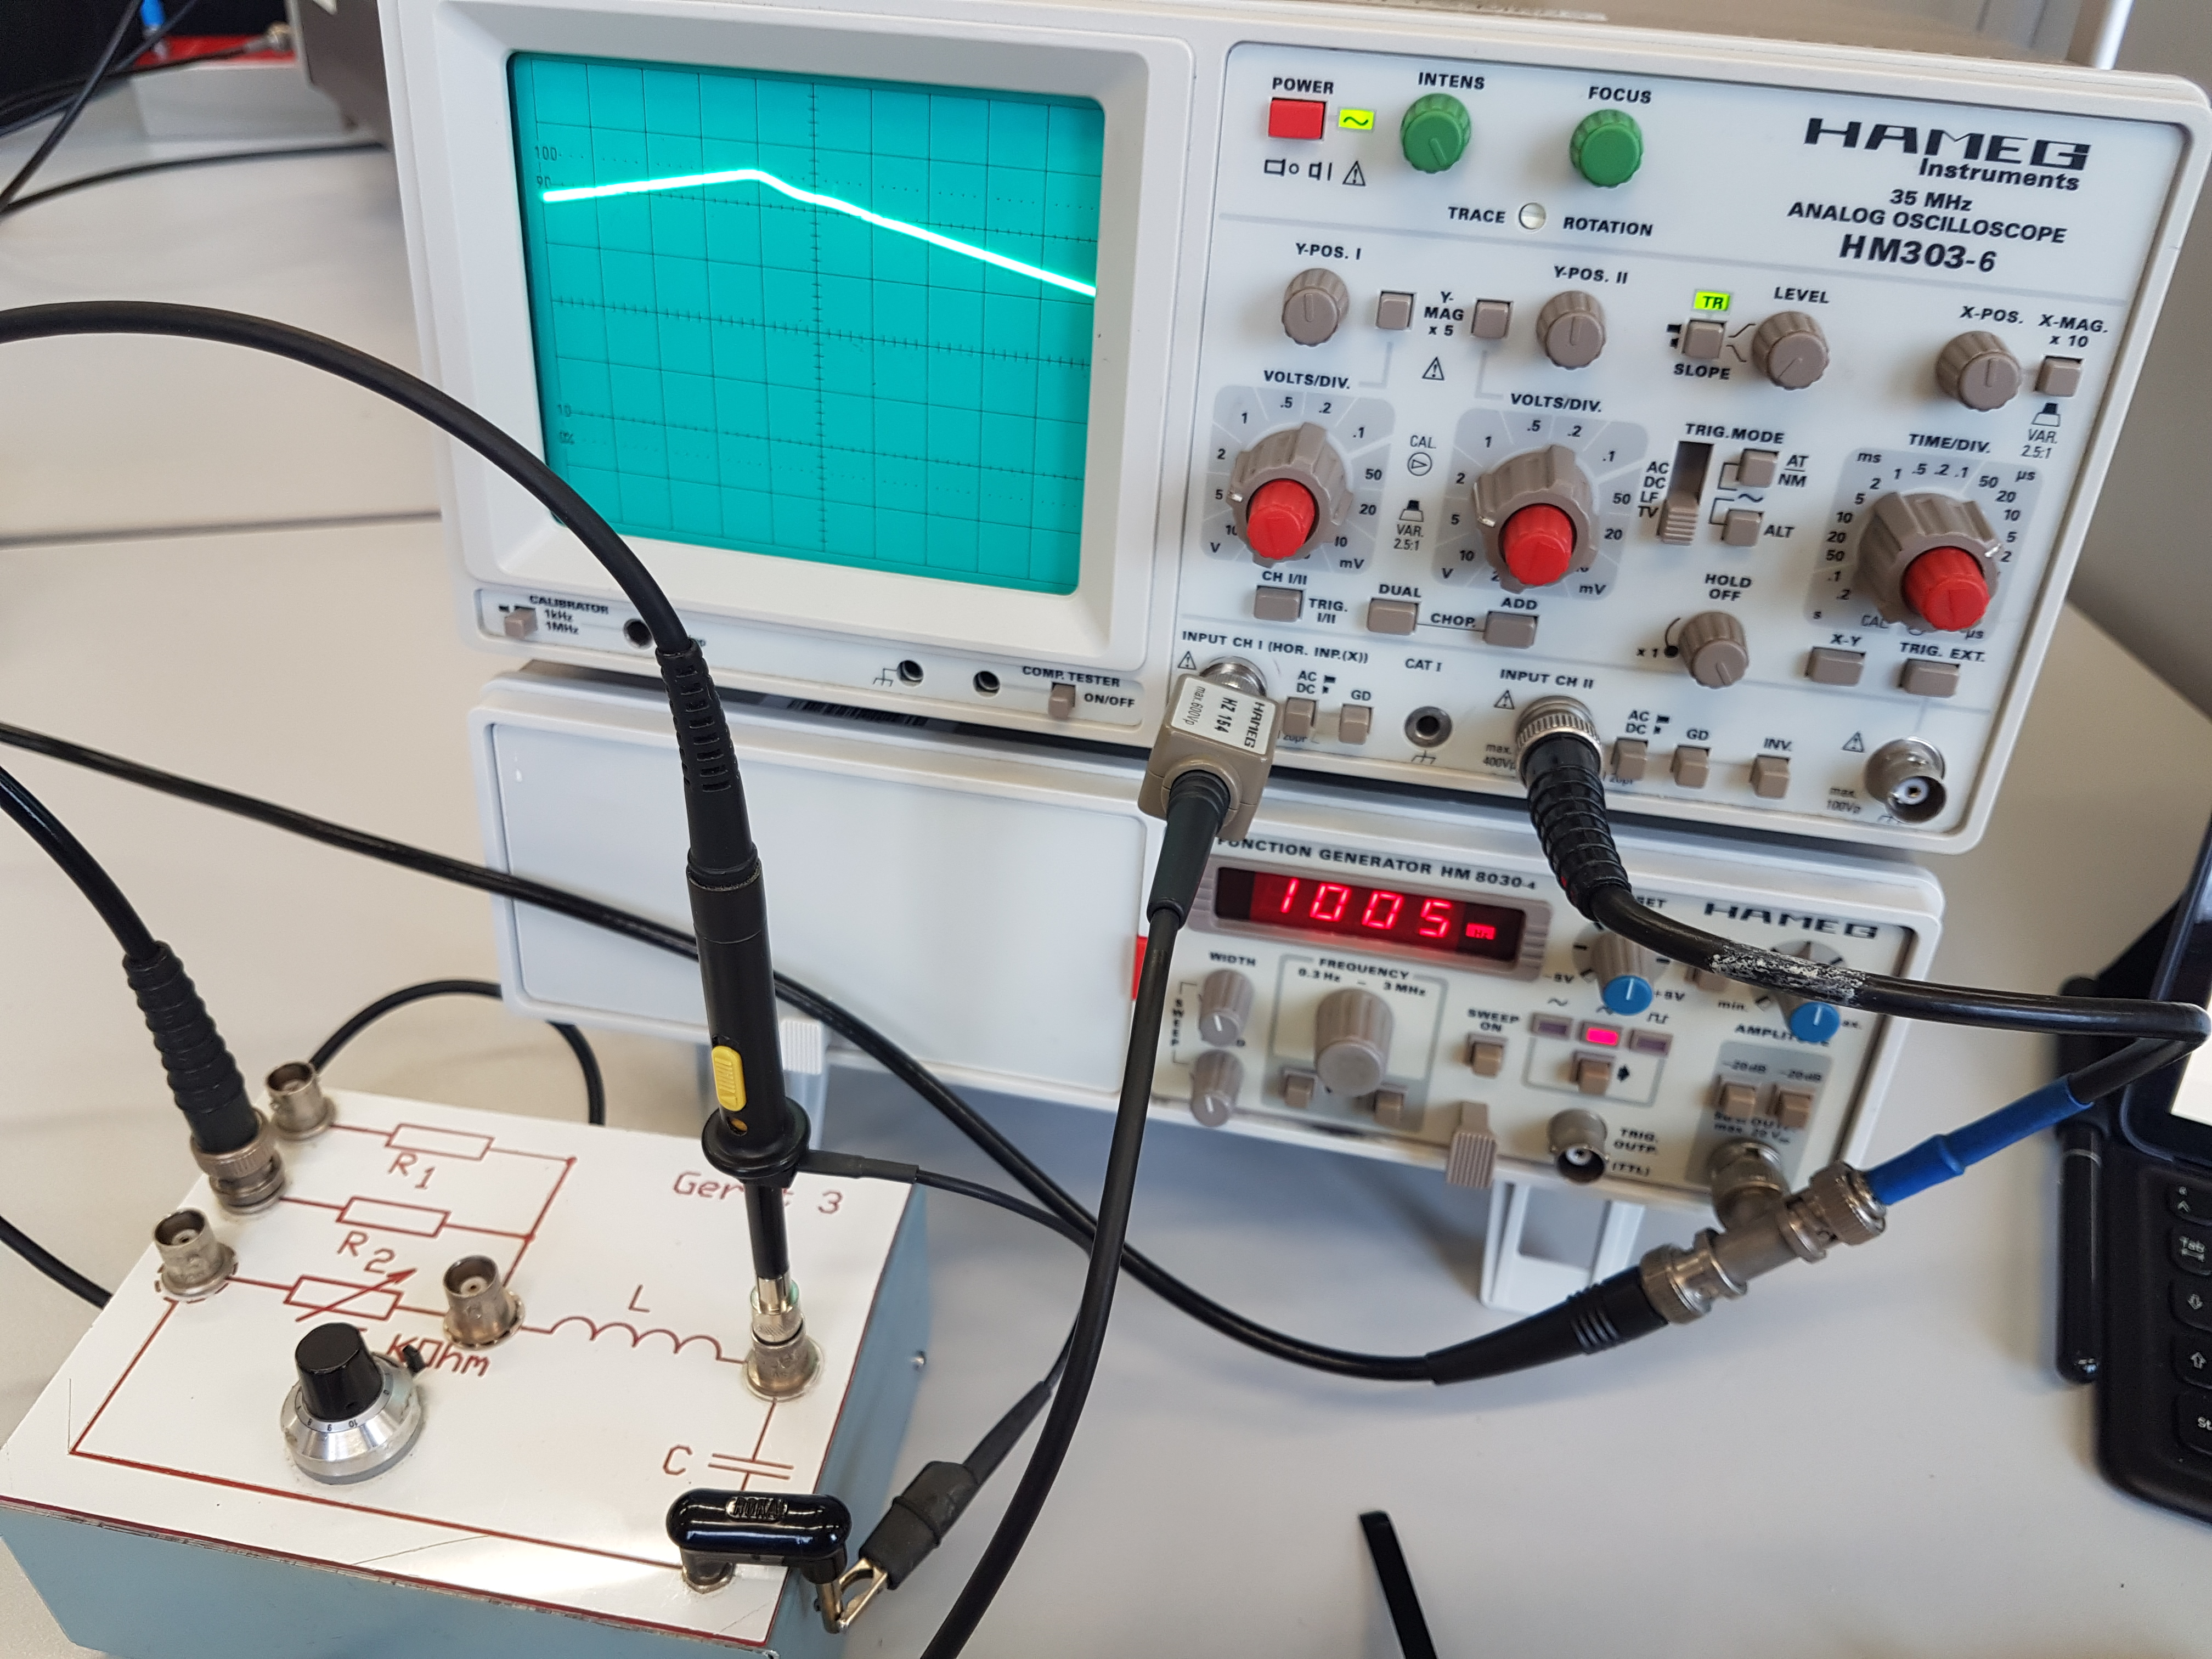
\includegraphics[width=\textwidth]{images/R2.jpg}
     \centering
     \caption{Widerstand R2}
     \label{fig:R2}
    \end{subfigure}




    \caption{Dämpfungsverhalten der Widerstände R1 und R2}
  \end{figure} 
  \begin{figure}[H]
    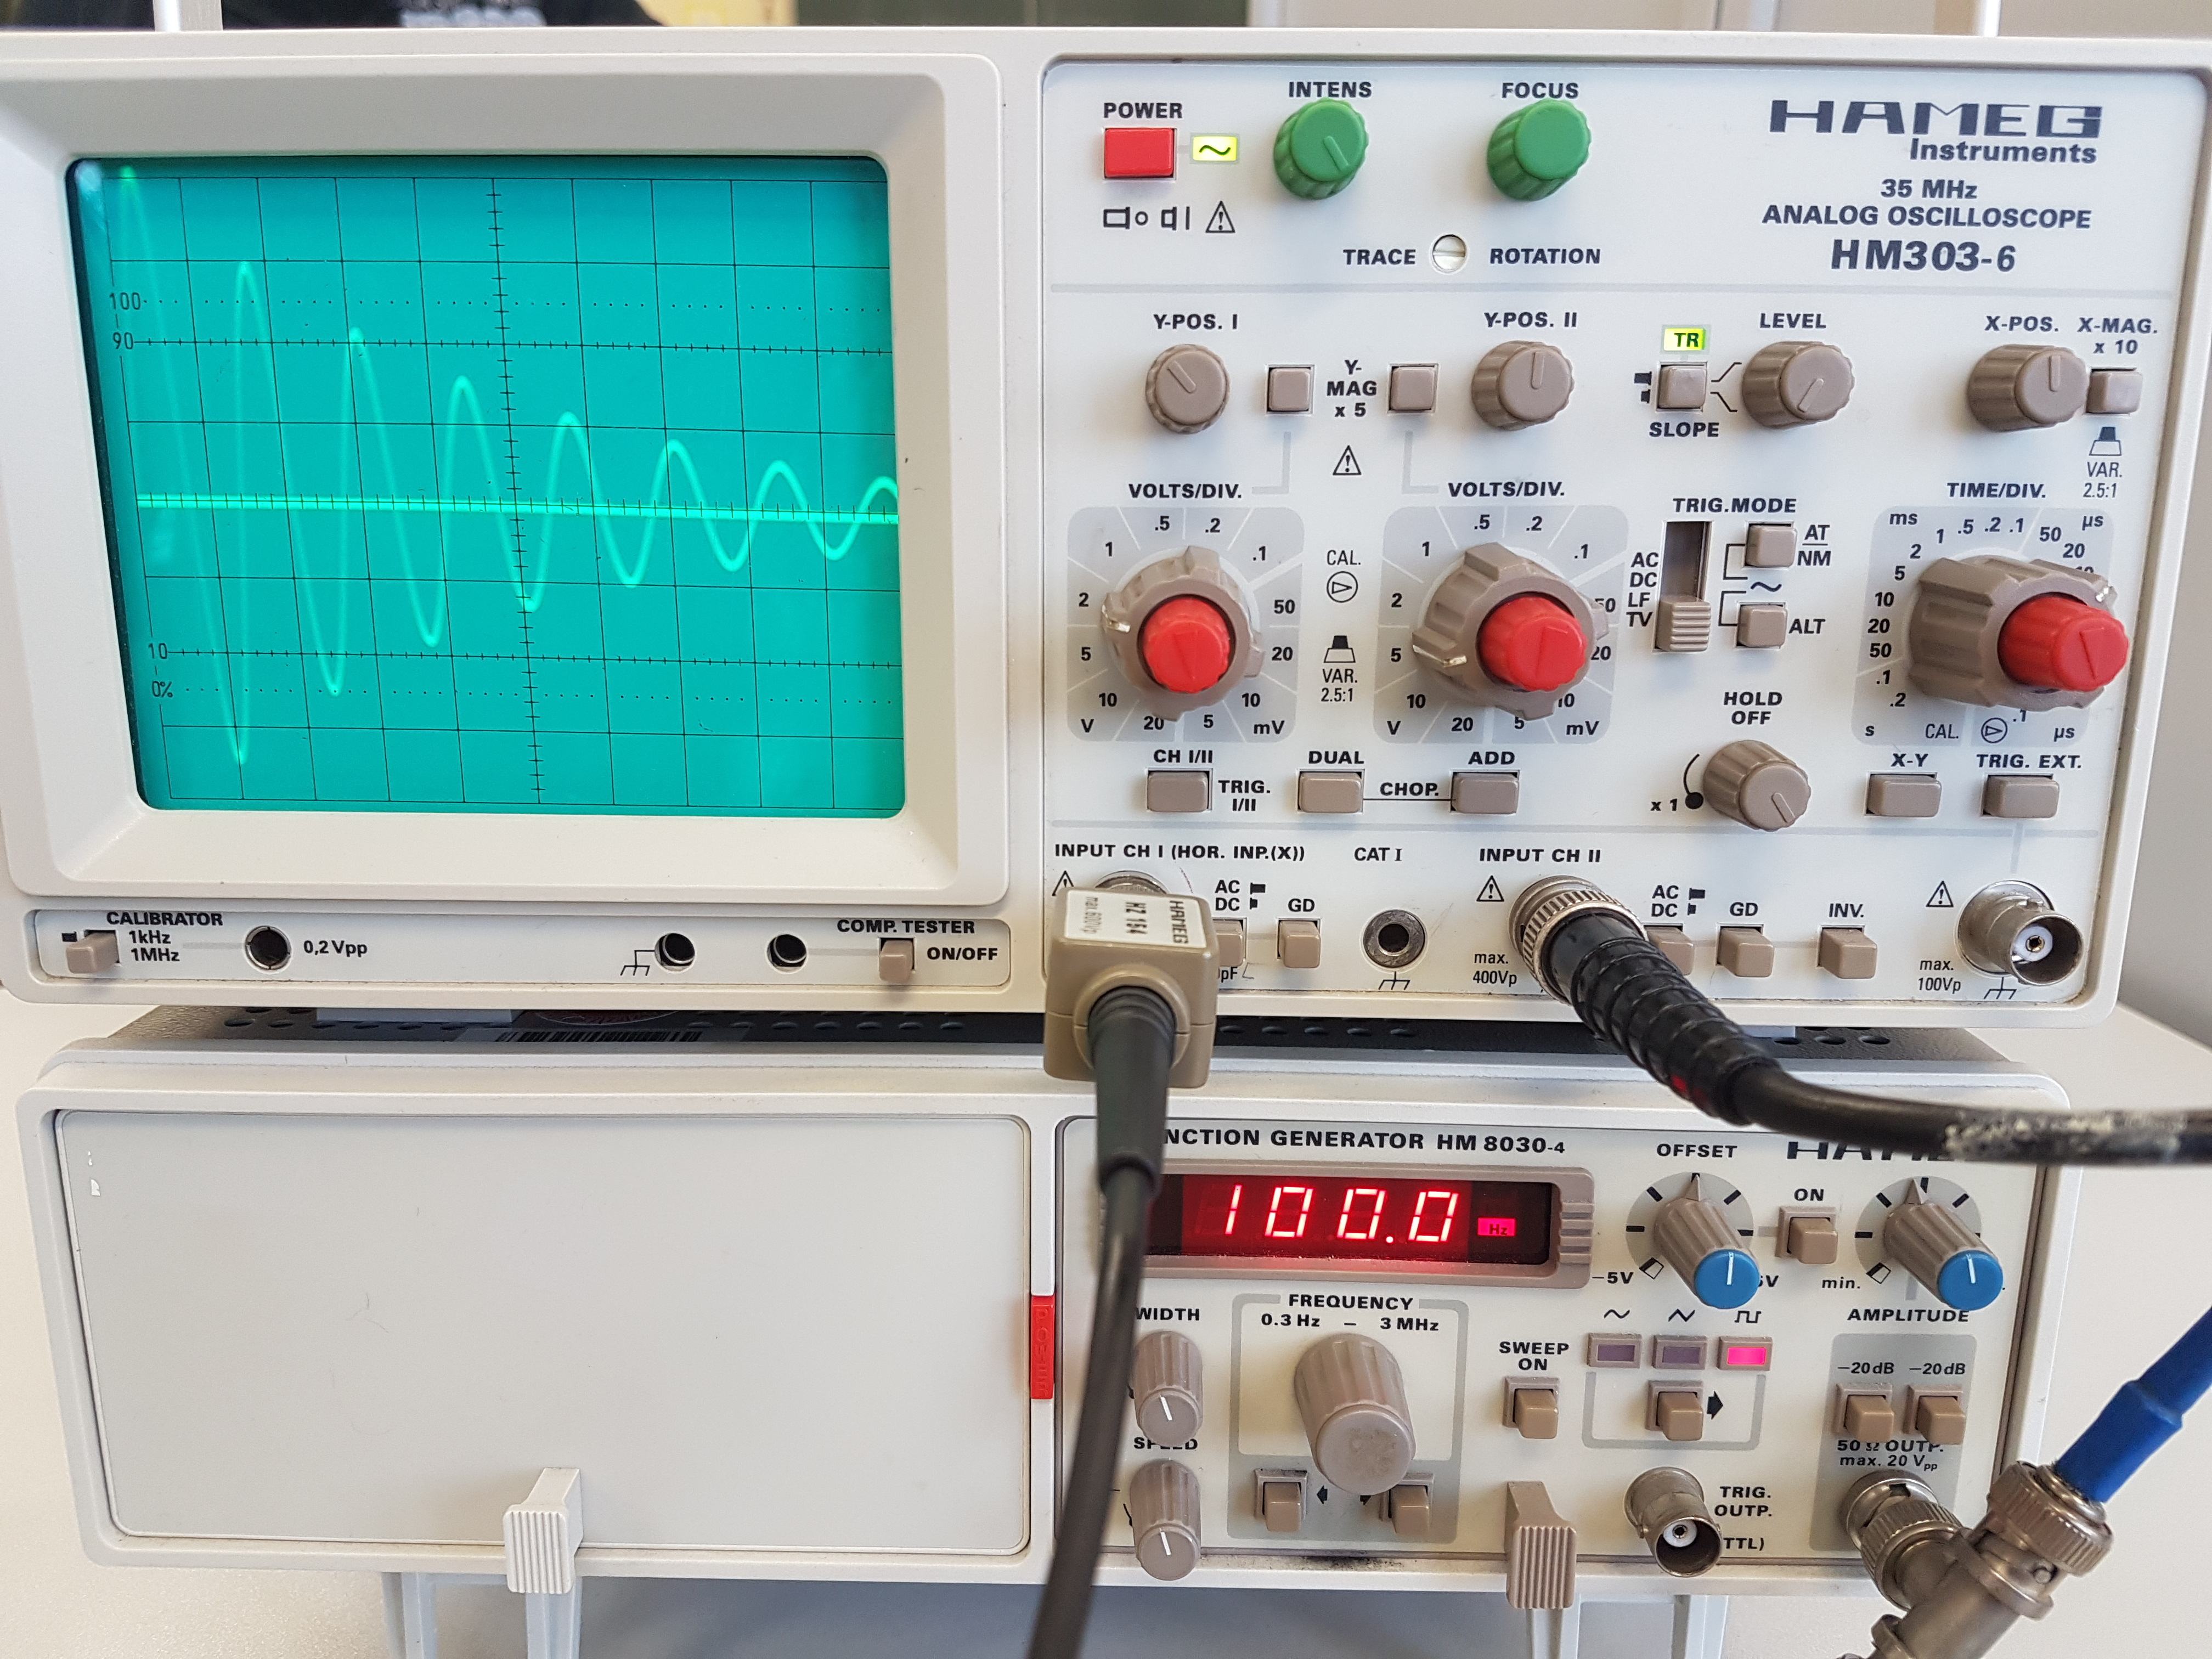
\includegraphics[width=0.75\textwidth]{images/5a.jpg}
    \centering
    \caption{Schwingungskurve für die Einhüllende}
    \label{fig:5a}
  \end{figure}
  \newpage

  \flushleft{Die }\justifying in Abbildung \ref{fig:5a} zu sehende Kurve beschreibt das Dämpfungsverhalten des LRC-Kreises bei einer angelegten Spannung von 
  10V, einem Widerstand von $\SI{271.6\pm0.2}{\ohm}$ und einer Frequenz von 100Hz. Aus Abbildung \ref{fig:5a} wurden die Amplituden der positiven Peaks
  abgelesen und in Tabelle \ref{tab:data_a} mit der zugehörigen Phasenverschiebung $t$ zusammengetragen.

  \begin{table}[H]
        \centering
        \caption{Messdaten von Aufg. a)}
        \input{table_a.tex} 
        \label{tab:data_a}
  \end{table}

  \flushleft{Mithilfe }\justifying der Messwertpaare lässt sich der folgende Graph \ref{fig:5ajpg} beschreiben, welcher die Einhüllende 
  Funktion $e^{-2\pi\mu t}$ des Schwingverhaltens als lineare Regression darstellt.\\
  Dabei ergibt sich die einhüllende Funktion aus Formel \eqref{eq:I}.\\
  Die ausgerechnten Werte von der Steigung $m$ und dem Schnittpunkt mit der y-Achse $b$ aus der Ausgleichsrechnung sehen dabei folgendermaßen aus:
  \begin{align}
      &m=\text{\input{m.tex}}
      &b=\text{\input{b.tex}}
  \end{align}
  \flushleft{Dabei }\justifying ist $m=-2\pi \mu$.

  \begin{figure}[H]
    \includegraphics[width=0.75\textwidth]{build/plota.pdf}
    \centering
    \caption{Lineare Regression der Einhüllenden}
    \label{fig:5ajpg}
  \end{figure}
  \newpage
  \begin{align}
    \intertext{\flushleft{Der} Wert für die Abklingdauer nach Formel \eqref{eq:Abkling} ergibt dabei:}
    T_{\text{ex}} &=\text{\input{T_ex.tex}}
    \intertext{Die aus den Theoriewerten erechnete Abklingdauer lautet:}
    T_{\text{ex,Lit.}}&=\text{\input{T_ex_lit.tex}}
  \end{align}
  Die Werte für den effektiven Widerstand lauten nach Gleichung \eqref{eq:Abkling} wie folgt:

\begin{align}
  &R_{\text{eff}}=\text{\input{R_eff.tex}} 
  &R_{\text{eff,Lit.}}=\text{\input{R1.tex} }
\end{align}


%Auswertung 5b ----------------------------------------------------------------------------------------------------------------------------------------

  \flushleft{Der }\justifying aus dem Experiment bestimmte Widerstand $R_{ap}$ des aperiodischen Grenzfalls lautet:
  \begin{equation}
  R_{\text{ap}} = \text{\input{Rap.tex}} \label{eq:Rap}
  \end{equation}
  Aus den Literaturwerten $L = \text{\input{L.tex}}$ und $C =\text{\input{C.tex}}$ ergibt sich der Widerstand 
  \begin{equation}
  R_{\text{ap, Lit.}} = \text{\input{R_ap_lit.tex}} \label{eq:RapLit}.
  \end{equation}

%Auswertung 5c ----------------------------------------------------------------------------------------------------------------------------------------

  \begin{table}[H]
        \centering
        \caption{Messdaten von c) und d)}
        \input{build/table_c.tex} 
        \label{tab:data_c}
  \end{table}

  \flushleft{Aus }\justifying den Messwertpaaren $(U_C, \nu)$ der Tabelle \ref{tab:data_c} werden zwei Graphen erstellt. Der erste Graph \ref{fig:5clin} 
  gibt den linearen Verlauf von Frequenz und Spannung wieder. Die waagerechte Gerade stellt $\sfrac{U_{C,\text{max}}}{\sqrt{2}}$ graphisch dar und diktiert
  die Breite der Resonanzkurve anhand der Schnittpunkte mit den Messwerten. Um dies zu verdeutlichen wurde die Breite der Resonanzkurve mit zwei vertikalen 
  Linien eingezeichnet. 


  \begin{figure}[H]
    \begin{subfigure}{0.495\linewidth}
     \includegraphics[width=\textwidth]{build/plotclin.pdf}
     \centering
     \caption{Lineare Darstellung}
     \label{fig:5clin}
    \end{subfigure}
    \begin{subfigure}{0.495\linewidth}
     \includegraphics[width=\textwidth]{build/plotcln.pdf}
     \centering
     \caption{Logarithmische Darstellung}
     \label{fig:5cln}
    \end{subfigure}
    \caption{Resonanzkurve aus Aufg. c)}
  \end{figure} 

  \flushleft{Die }\justifying Theorie- und Ausgleichskurve wurden dabei mit der Formel \eqref{eq:9} erstellt,
  wobei $U_0$ vorher noch auf die linke Seite der Gleichung multipliziert wurde.
  Die Fitparameter sehen dabei folgendermaßen aus:
  \begin{subequations}
  \begin{align}
    R &= \SI{1.23}{\kilo\ohm}\\
    L &= \SI{3.97}{\milli\henry}\\
    C &= \SI{2.76}{\nano\farad}.
  \end{align}
  \end{subequations}

  \flushleft{Bestimmt }\justifying wurde die Breite der Resonanzkurve $\omega_+ - \omega_-$ mit $\omega = 2\cdot\pi\cdot\nu$ 
  und der Formel \eqref{eq:om+-}. Der errechneten Werte für $\omega_+ - \omega_-$ und $\omega_{+-,\text{Lit.}}$ sehen aus wie folgt:
   
  \begin{align}
  \omega_+ - \omega_- &= \text{\input{nuGraph.tex}} \label{eq:28}\\
  \omega_{+-,\text{Lit.}} &= \text{\input{nuRech.tex}} \label{eq:29}
  \end{align}

  \flushleft{Aus }\justifying dem Graphen \ref{fig:5clin} und der Formel \eqref{eq:guete} ergibt sich die errechnete Resonanzüberhöhung von
  \begin{align}
  q &= \text{\input{q.tex}} \label{eq:33}
  \intertext{mit dem Literaturwert}
  q_{\text{Lit.}} &= \text{\input{q_lit.tex}}. \label{eq:34}
  \end{align}
  \newpage
  
%Auswertung 5d ----------------------------------------------------------------------------------------------------------------------------------------

  \flushleft{Mit }\justifying den Messwertpaaren $(t, \nu)$ aus Tabelle \ref{tab:data_c} lassen sich die folgenden zwei Graphen erstellen:

  \begin{figure}[H]
    \begin{subfigure}{0.495\linewidth}
     \includegraphics[width=\textwidth]{build/plotdlin.pdf}
     \centering
     \caption{Lineare Darstellung}
     \label{fig:4dlin}
    \end{subfigure}
    \begin{subfigure}{0.495\linewidth}
     \includegraphics[width=\textwidth]{build/plotdln.pdf}
     \centering
     \caption{Logarithmische Darstellung}
     \label{fig:4dln}
    \end{subfigure}
    \caption{Resonanzkurve aus Aufg. 4d)}
  \end{figure} 

  \flushleft{Die\;}Theoriekurve und die gefittete Kurve wurden hier mit der Formel \eqref{eq:phi} erstellt. Die Fitparameter
  sehen dabei folgendermaßen aus:
  \begin{align}
    R&= \SI{4.71}{\kilo\ohm}\\
    L&= \SI{-136}{\milli\henry}\\
    C&= \SI{-99.7}{\pico\farad}
  \end{align}

  \flushleft{Mithilfe }\justifying der Formel \eqref{eq:omegares} wird der Wert für $\nu_{\text{res.}}$ berechnet. Anhand $\nu_{\text{res.}}$
  können die Werte für $\nu_{1,2}$ bestimmt werden, indem die Funktionswerte bei $\sfrac{\pi}{2}$ und 
  $\sfrac{3\pi}{2}$ betrachtet werden. Demnach folgen aus Formeln \eqref{eq:omegares} und \eqref{eq:om12} die Werte für $\nu_{1,2,\text{res.}}$ und die
  zugehörigen Literaturwerte:
  \begin{subequations}\label{eq:36}
  \begin{align}
    &\nu_1 = \text{\input{nu1.tex}} \qquad &\nu_{1,\text{Lit.}} &= \text{\input{nu1_lit.tex}} \\
    &\nu_2 = \text{\input{nu2.tex}} \qquad &\nu_{2,\text{Lit.}} &= \text{\input{nu2_lit.tex}} \\
    &\nu_{\text{res.}} = \text{\input{nu_res.tex}} &\qquad \nu_{\text{res.,Lit.}} &= \text{\input{nu_res_lit.tex}}
  \end{align}
  \end{subequations}
  \newpage

% Diskussion %%%%%%%%%%%%%%%%%%%%%%%%%%%%%%%%%%%%%%%%%%%%%%%%%%%%%%%%%%%%%%%%%%%%%%%%%%%%%%%%%%%%%%%%%%%%%%%%%%%%%%%%%%%%%%%%%%%%%%%%%%%%%%%%%%%%%%%%%%%

\section{Diskussion}\justifying

\flushleft{Die }\justifying Kurve der gemessen Werte für a) liegt nahe der erwarteten Kurve aus der Theorie. Bei einer angelegten 
Spannung von 10V wird der Logarithmus der Maximalamplitude $\log{U_{max}} = \num{2.3} $ erwartet. Die Maximalamplitude aus Tabelle \ref{tab:data_a}, 
welche kleiner als 2.3V ist, ließe sich durch einen weiteren Peak mit einer negativen Amplitude erklären, der nicht auf dem Bild 
\ref{fig:5a} aufgeführt ist. Die Werte für die Abklingdauer und den effektiven Widerstand haben allerdings einen relativ hohen Fehler,
\begin{align}
  \frac{T_{\text{ex}}-T_{\text{ex,Lit.}}}{T_{\text{ex,Lit.}}}&=\text{\input{RF_T_ex.tex}},\\
  \frac{R_{\text{eff}}-R_{\text{eff,Lit.}}}{R_{\text{eff,Lit.}}}&= \text{\input{RF_R_eff.tex}},
\end{align}
welcher sich eventuell auf systematische Fehler zurückführen ließe. 

\flushleft{Der }\justifying für b) berechnete Widerstand \eqref{eq:Rap} zeigt einen hohen relativen Fehler von 
\begin{align}
  \frac{R_{\text{ap}}-R_{\text{pap,Lit.}}}{R_{\text{ap,Lit.}}}= \text{\input{RF_R.tex}}.
\end{align}

\flushleft{Dieser\;}\justifying könnte durch die fehlerhafte Interpretation der Skalierung des variablen Widerstandes erklärt werden. Denn die Skalaierung 
des Widerstandes verlief von null bis zehn, wohingegen der maximale Widerstand bei $\SI{5.0}{\kilo\ohm} $ lag. Dieser Umstand wirft die 
Vermutung auf, dass die Skalierung $\SI{0.5}{\kilo\ohm}$ pro Einheit betrug, anstelle der hier verwendeten $\SI{1}{\kilo\ohm} $ pro Einheit. Demnach 
würde der Widerstand $R_{\text{ap}} = \SI{1.45}{\kilo\ohm}$ entsprechen, was deutlich näher am Theoriewert läge.

\flushleft{Die }\justifying für c) erhobenen Messwerte geben im Graphen \ref{fig:5clin} die Resonanzkurve eines Bandpasses wieder.
Dabei entspricht die gefittete Kurve überhaupt nicht den Messwerten. Auch der theoretisch erwarteten Kurve entspricht sie nicht, da die Breite der Resonanzkurve zu
schmal ist nach Gleichung \eqref{eq:29}. Eine Möglichkeit für den misslungenen Plot können
systematische Fehler sein oder aber, dass die Gleichung \eqref{eq:9} nicht als Fitfunktion
geeignet ist.
Es lässt sich eindeutig eine schwache Dämpfung erkennen, da das Amplitudenmaximum die 1V überschreitet. Bei der Betrachtung der relativen
Fehler von der Resonanzüberhöhung $q$ \eqref{eq:33} 
\begin{align}
\frac{q - q_{\text{lit}}}{q_{\text{lit}}}&= \text{\input{RF_q.tex}}
\intertext{und $\omega _+ - \omega_-$ \eqref{eq:28}}
\frac{\omega_{+-} - \omega_{+-,\text{Lit.}}}{\omega_{+-,\text{Lit.}}} &= \text{\input{RF_nu.tex}} \qquad \qquad \text{mit} \; \omega_{+-} = \omega_+ - \omega_-
\end{align}
zeigen sich signifikante Fehler von $-22\%$ und $19\%$.
Diese Fehler könnten auf einen systematischen 
Fehler zurückgeführt werden.

\flushleft{Die\;}\justifying im Graphen \ref{fig:4dln} gefittete Kurve entspricht nicht den Messwerten.
Die Ursache hierbei liegt höchstwahrscheinlich daran, dass die Gleichung \eqref{eq:phi} unsere Kurve nicht
beschreiben kann. Dies sieht man daran, dass der Wertebereich der Funktion sich nur von $\sfrac{-\pi}{2} $ bis
$\sfrac{\pi}{2} $ erstreckt. Folglich müsste die Funktion der Theorie zufolge auch in $\sfrac{3\pi}{2} $ definiert sein.

\flushleft{Aus }\justifying den für d) berechneten Werten für $\nu_{1,2,\text{res.}}$ \eqref{eq:36} und deren relativen Fehlern von
  \begin{subequations}\label{eq:37}
  \begin{align}
    \frac{\nu_1 - \nu_{1,\text{Lit.}}}{\nu_{1,\text{Lit.}}} &= \text{\input{RF_nu1.tex}}, \\
    \frac{\nu_2 - \nu_{2,\text{Lit.}}}{\nu_{2,\text{Lit.}}} &= \text{\input{RF_nu2.tex}} \text{und} \\
    \frac{\nu_{\text{res.}} - \nu_{\text{res.,Lit.}}}{\nu_{\text{res.,Lit.}}} &= \text{\input{RF_nu_res.tex}}
  \end{align} 
  \end{subequations}
lässt sich entnehmen, dass die errechneten Werte jeweils sehr nahe an den Literaturwerten liegen. Demnach folgt aus den geringen Abweichungen, in 
Verbindung mit den Formeln \eqref{eq:omega0} und \eqref{eq:om12}, dass es sich hier um eine starke Dämpfung handeln könnte.

\flushleft{Mit }\justifying den Erkenntnissen aus Aufgaben c) und d) lässt sich vermuten, dass das vorliegende System nach Formel 
\eqref{eq:Fall2b} der starken Dämpfung sehr nahe liegt.  

\newpage

\printbibliography
\end{document}




